%===============Synopsis by C. Has=================================
\documentclass[11pt, a4paper]{article}

\usepackage[T1]{fontenc}
\usepackage{times}
\usepackage{graphicx}\graphicspath{{gfx/}}
\usepackage[margin=1in]{geometry}
\usepackage[onehalfspacing]{setspace}
\usepackage{caption,subcaption}
\usepackage[sort&compress, numbers]{natbib}
\captionsetup{font={small, stretch=1}}
\usepackage[colorlinks]{hyperref}
\usepackage{cleveref}
\usepackage{pdfpages}
%==================================================================

\title{\vskip-2.5cm Place the Title of Your Synopsis Report\vskip-5mm}
\author{Author name\\ Department name. Institute name, Place, Country}\date{}

\begin{document}
\maketitle\hrule

\tableofcontents

\section{Introduction}\label{sec:intro}
LaTeX is a high-quality typesetting system; it includes features designed for the production of technical and scientific documentation. LaTeX is the de facto standard for the communication and publication of scientific documents. LaTeX is available as free software.

LaTeX is widely used in academia for the communication and publication of scientific documents in many fields, including mathematics, statistics, computer science, engineering, chemistry, physics, economics, linguistics, quantitative psychology, philosophy, and political science. It also has a prominent role in the preparation and publication of books and articles that contain complex multilingual materials, such as Tamil, Sanskrit and Greek. LaTeX uses the TeX typesetting program for formatting its output, and is itself written in the TeX macro language.

LaTeX is intended to provide a high-level language that accesses the power of TeX in an easier way for writers. In short, TeX handles the layout side, while LaTeX handles the content side for document processing. LaTeX comprises a collection of TeX macros and a program to process LaTeX documents. Because the plain TeX formatting commands are elementary, it provides authors with ready-made commands for formatting and layout requirements such as chapter headings, footnotes, cross-references and bibliographies.

In order to create a document in LaTeX, you first write a file, say document.tex, using your preferred text editor. Then you give your document.tex file as input to the TeX program (with the LaTeX macros loaded), and TeX writes out a file suitable for viewing onscreen or printing. This write-format-preview cycle is one of the chief ways in which working with LaTeX differs from what-you-see-is-what-you-get word-processing. It is similar to the code-compile-execute cycle familiar to computer programmers. Today, many LaTeX-aware editing programs make this cycle a simple matter of pressing a single key, while showing the output preview on the screen beside the input window. Some online LaTeX editors automatically refresh the preview. Other online tools provide incremental editing in-place, mixed in with the preview in a streamlined single window.

\subsection{Figures}
A useful extension is the subcaption (\Cref{fig:subfigs cap}) package, which uses subfloats within a single float. The subfig package (subfigure package is deprecated) is a useful alternative when used in-conjunction with LaTeX templates (i.e. templates for journals from Springer and IOP, IEEETran and ACM SIG) that are not compatible with subcaption. These packages give the author the ability to have subfigures within figures, or subtables within table floats. Subfloats have their own caption, and an optional global caption.

\begin{figure}
	\centering
	\begin{subfigure}[b]{0.45\linewidth}
		\centering
		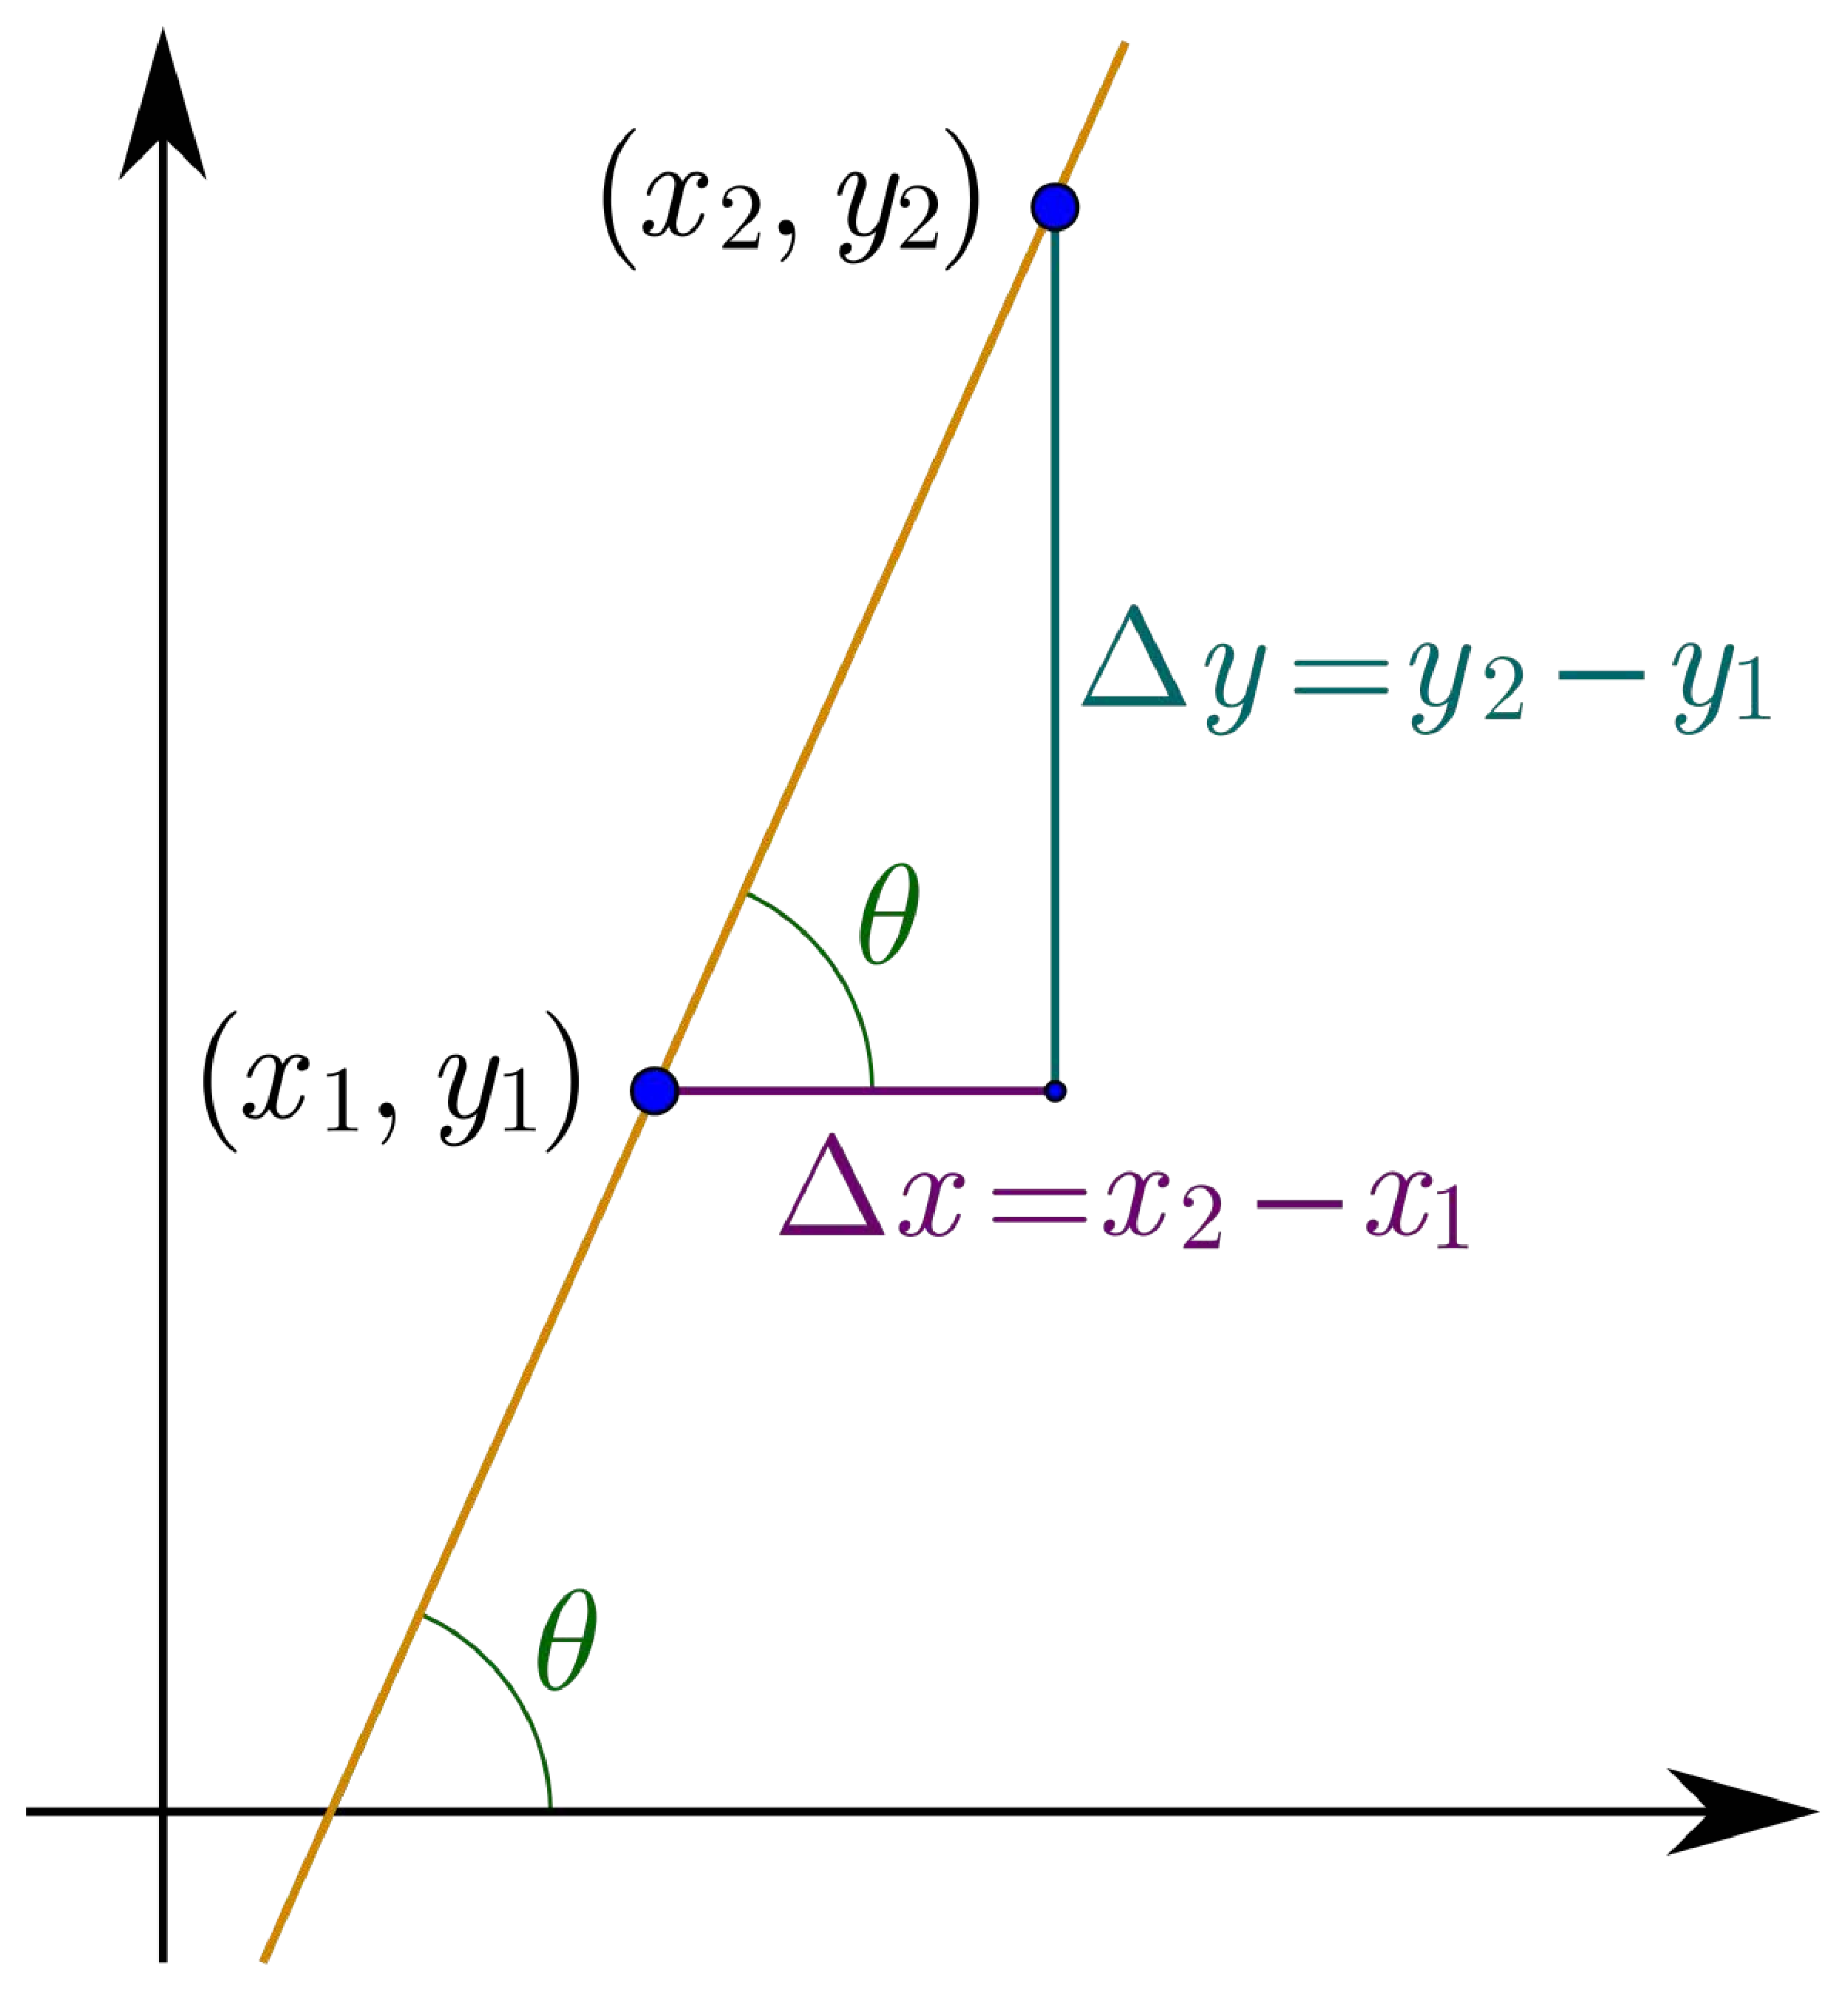
\includegraphics[width=0.75\linewidth]{slope}
		\caption{}
		\label{fig:slope}
	\end{subfigure}
	~
	\begin{subfigure}[b]{0.45\linewidth}
		\centering
		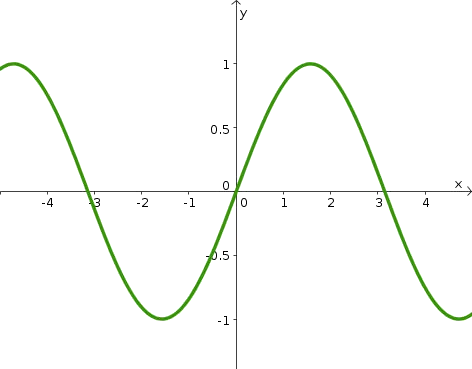
\includegraphics[width=\linewidth]{sine-graph}
		\caption{}
		\label{fig:sine-graph}
	\end{subfigure}
	\caption{An example of how to place two figures side by side using subcaption package. (a) Slope of a straight line, and (b) an illustration of a sinusoidal curve.}
	\label{fig:subfigs cap}
\end{figure}

\subsection{Table}
Tables are a common feature in academic writing, often used to summarize research results. Mastering the art of table construction in LaTeX is therefore necessary to produce quality papers and with sufficient practice one can print beautiful tables of any kind.

Keeping in mind that LaTeX is not a spreadsheet, it makes sense to use a dedicated tool to build tables and then to export these tables into the document. Basic tables are not too taxing, but anything more advanced can take a fair bit of construction; in these cases, more advanced packages can be very useful. However, first it is important to know the basics. Once you are comfortable with basic LaTeX tables, you might have a look at more advanced packages or the export options of your favorite spreadsheet. Thanks to the modular nature of LaTeX, the whole process can be automated in a fairly comfortable way (\Cref{tab:sample2}).

\begin{table}
	\centering
	\caption{Place the caption for this table.}
	\label{tab:sample2}
	\renewcommand{\arraystretch}{1.5}
	\begin{tabular*}{\linewidth}{c @{\extracolsep{\fill}} ccccccc}
		\hline 
		Data 1 & Data 2 & Data 3 & Data 4 & Data 5 & Data 6 & Data 7 & Data 8\\ \hline
		a & b & c & d & b & c & d & b \\ 
		5 & 6 & 7 & 8 & b & c & d & b \\ 
		9 & 10 & 11 & 12 & b  & c & d & e \\ 
		a & b & c & d & b & c & d & b \\ 
		5 & 6 & 7 & 8 & b & c & d & b \\ 
		9 & 10 & 11 & 12 & b & c  & d & b \\ 
		a & b & c & d & b & c & d & b \\ \hline 
	\end{tabular*} 
\end{table}

\section{Literature}\label{sec:lit}
Literature, most generically, is any body of written works. More restrictively, literature refers to writing considered to be an art form or any single writing deemed to have artistic or intellectual value, often due to deploying language in ways that differ from ordinary usage.

\subsection{Equation}
One of the greatest motivating forces for Donald Knuth when he began developing the original TeX system was to create something that allowed simple construction of mathematical formulae, while looking professional when printed. The fact that he succeeded was most probably why TeX (and later on, LaTeX) became so popular within the scientific community. Typesetting mathematics is one of LaTeX's greatest strengths. It is also a large topic due to the existence of so much mathematical notation. As~\Cref{eq: momentum diff} shows how to label any equation in latex. 

The velocity, v ($v=d/t$) is ....
%
\begin{equation}\label{eq: momentum diff}
\nu = \frac{\mu}{\rho}
\end{equation}

\subsection{Hpw to cite?}
Citations are referred in the text using \verb|\citet| command which produces citations
as they are part of the text. In order to say somebody did this work as a part of a line use: \verb|\citet{voet2011biochemistry}| have done extensive work on .... This will produce~\citet{voet2011biochemistry} have done extensive work on .... Alternately citations can appear in parenthesis. The command~\verb|\citep| is used to automatically put the citations in parenthesis. As an example, consider the extensive work done in the area of book writing~\citep{seifert1991shape}.
Article~\citep{sircar1972adsorption,keh1995particle} and collection of work~\citep{seifert1995morphology} are the other examples.

\section{Experimental work}\label{sec:exp}

\subsection{First subsection}
An experiment is a procedure carried out to support, refute, or validate a hypothesis. Experiments provide insight into cause-and-effect by demonstrating what outcome occurs when a particular factor is manipulated. Experiments vary greatly in goal and scale, but always rely on repeatable procedure and logical analysis of the results. There also exists natural experimental studies.

\begin{figure}
	\centering
	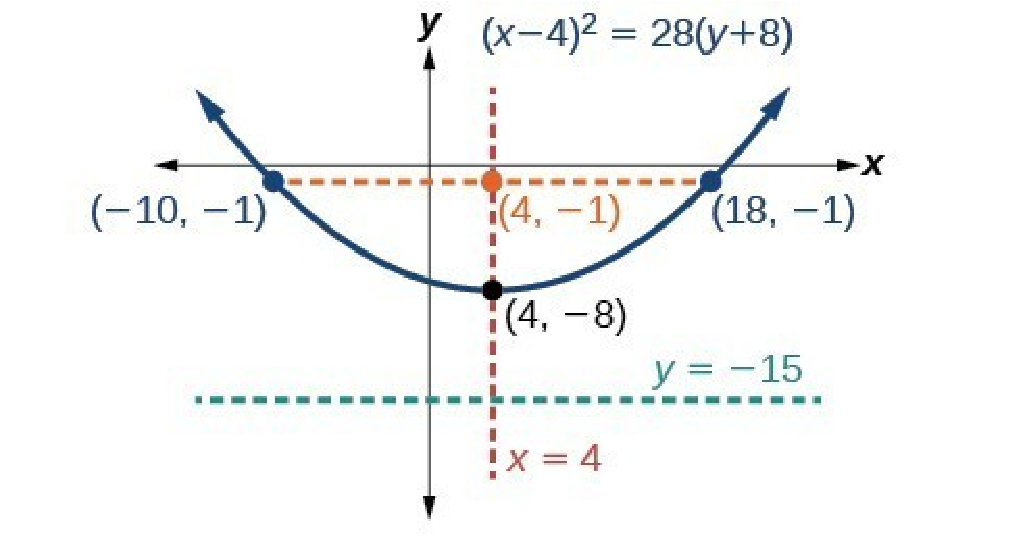
\includegraphics[width=0.45\linewidth]{parabolic}
	\caption{Caption of Figure 1.}
	\label{fig:parabolic}
\end{figure}

A child may carry out basic experiments to understand gravity, while teams of scientists may take years of systematic investigation to advance their understanding of a phenomenon. Experiments and other types of hands-on activities are very important to student learning in the science classroom. Experiments can raise test scores and help a student become more engaged and interested in the material they are learning, especially when used over time. Experiments can vary from personal and informal natural comparisons (e.g. tasting a range of chocolates to find a favorite), to highly controlled (e.g. tests requiring complex apparatus overseen by many scientists that hope to discover information about subatomic particles). Uses of experiments vary considerably between the natural and human sciences.~\Cref{fig:parabolic} is the parabolic plot.

\subsubsection{First subsubsection}
An experiment usually tests a hypothesis, which is an expectation about how a particular process or phenomenon works. However, an experiment may also aim to answer a ``what-if'' question, without a specific expectation about what the experiment reveals, or to confirm prior results. If an experiment is carefully conducted, the results usually either support or disprove the hypothesis. According to some philosophies of science, an experiment can never "prove" a hypothesis, it can only add support. On the other hand, an experiment that provides a counterexample can disprove a theory or hypothesis, but a theory can always be salvaged by appropriate ad hoc modifications at the expense of simplicity. An experiment must also control the possible confounding factors—any factors that would mar the accuracy or repeatability of the experiment or the ability to interpret the results~(\Cref{app:liposyn}). Confounding is commonly eliminated through scientific controls and/or, in randomized experiments, through random assignment.

In engineering and the physical sciences, experiments are a primary component of the scientific method. They are used to test theories and hypotheses about how physical processes work under particular conditions (e.g., whether a particular engineering process can produce a desired chemical compound). Typically, experiments in these fields focus on replication of identical procedures in hopes of producing identical results in each replication. Random assignment is uncommon. 

\paragraph{Paragraph tile.}
According to his explanation, a strictly controlled test execution with a sensibility for the subjectivity and susceptibility of outcomes due to the nature of man is necessary.

\section{Conclusions}\label{sec:conc} 
Conclusions show readers the value of your completely developed argument or thoroughly answered question. Consider the conclusion from the reader's perspective. At the end of a paper, a reader wants to know how to benefit from the work you accomplished in your paper. 

%\section{Supporting information}
%The purpose of the supporting information is to enable authors to provide and archive supporting information such as data tables, method information, figures, video, or computer software, in digital formats so that other scientists can use it.

\small\singlespacing
\bibliographystyle{unsrtnat} 
\bibliography{mybib} 

\appendix
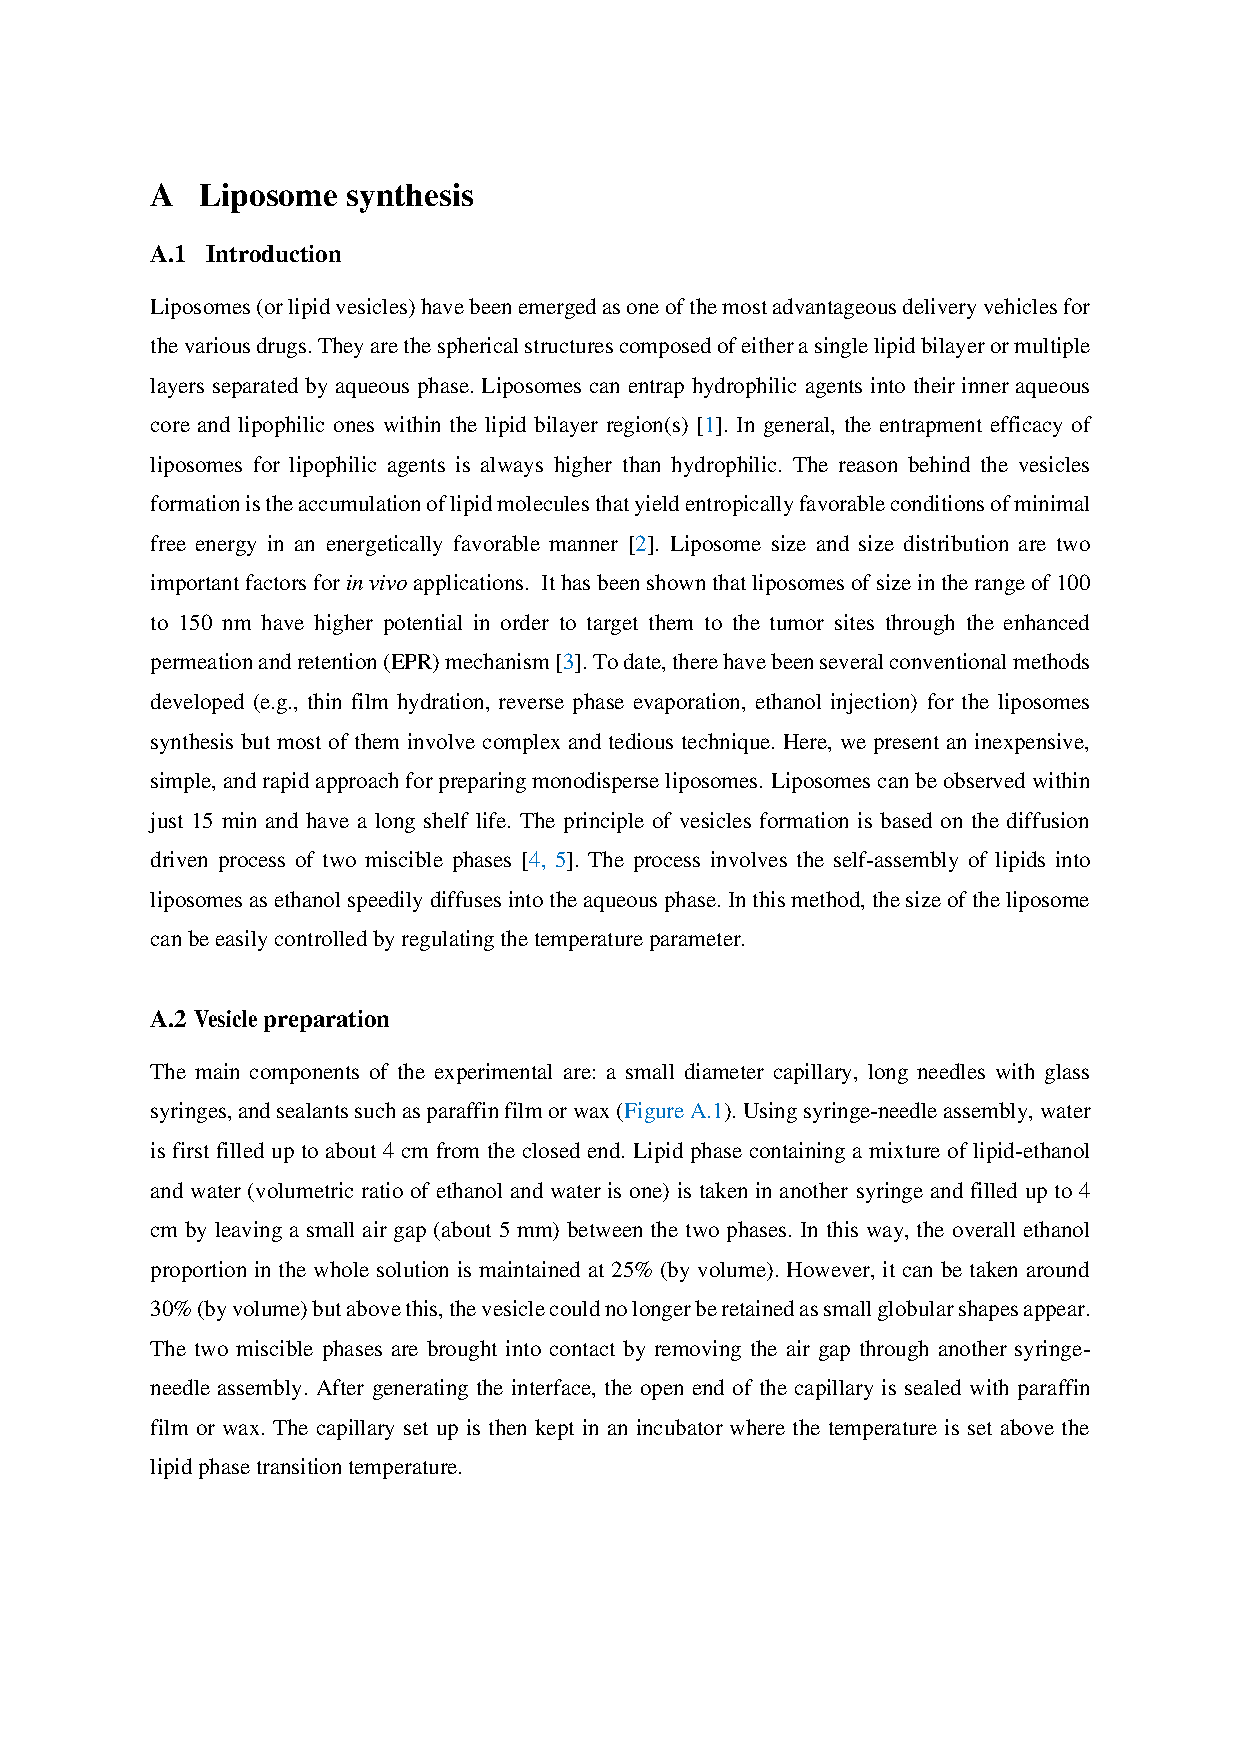
\includepdf[pages=1-3, pagecommand={\thispagestyle{plain}},
addtotoc={1, section, 1, Liposome synthesis, app:liposyn,
	1, subsection, 2, Introduction, subapp:intro,
	1, subsection, 2, Vesicle preparation, subapp:vesprep,
	2, section, 1, Microfluidic device for generating solute gradients, app:microfluidics,
	2, subsection, 2, Introduction, subapp:micro}
]{external-docs/supporting-info}

\end{document}

%\addtotoc={page number, section, section level, title, label}
%
%section level: section: 1, subsection: 2, 

































